% Keep these two lines in order for typesetting to work w/ the funny fonts.
%!TEX TS-program = xelatex
%!TEX encoding = UTF-8 Unicode

\documentclass[11pt]{article}
\usepackage[margin=1.25in]{geometry}
\usepackage[config, font=small, labelfont={sf,bf}, textfont=sf]{caption,subfig}
\usepackage{graphicx}
\usepackage{hyperref}
\usepackage{amssymb}
\usepackage{hyperref}
\hypersetup{
    colorlinks,
    citecolor=black,
    filecolor=black,
    linkcolor=black,
    urlcolor=black
}
\usepackage{fontspec,xltxtra,xunicode}
\usepackage{setspace}
\setcounter{tocdepth}{2}
\defaultfontfeatures{Mapping=tex-text}
%\setromanfont[Mapping=tex-text]{Baskerville}
%\setromanfont{Fanwood Text}
\setromanfont{PT Serif}
%\setsansfont[Scale=MatchLowercase,Mapping=tex-text]{Gill Sans}
%\setsansfont[Scale=MatchLowercase]{Cabin}
%\setmonofont[Scale=MatchLowercase]{Andale Mono}
%\usepackage[margin=10pt,font=sf,labelfont=bf, labelsep=endash]{caption}

%% \usepackage{titlesec}
%% \newfontfamily\sectionfont{League Gothic}
%% \titleformat*{\title}{\Huge\bfseries\sffamily}
%% \titleformat*{\section}{\Huge\bfseries\sffamily}
%% \titleformat*{\subsection}{\Large\bfseries\sffamily}
%% \titleformat*{\subsubsection}{\large\bfseries\sffamily}

\newcommand{\sectionline}{%
  \vspace{\baselineskip}%
  \hspace{\fill}\rule{0.5\linewidth}{.7pt}\hspace{\fill}%
  \par \vspace{\baselineskip}
}

\newenvironment{packed_enum}{
\begin{enumerate}
  \setlength{\itemsep}{1pt}
  \setlength{\parskip}{0pt}
  \setlength{\parsep}{0pt}
}{\end{enumerate}}

\newenvironment{indentwholepara}[1]
{\begin{list}{}
         {\setlength{\leftmargin}{#1}}
         \item[]
}
{\end{list}}

\title{Thesis Proposal:\\ Interaction Techniques for Sketch-based
  Design} \author{Gabe Johnson\\School of Architecture\\Carnegie
  Mellon University\\ \\ (This is a draft)}

\begin{document}
\thispagestyle{empty}
\maketitle
\vspace{70pt}
\begin{center}Committee\\
\vspace{24pt}
\rule{0.8\linewidth}{0.7pt}
\\
\vspace{24pt}
\textit{Mark D. Gross} (Chair) --- School of Architecture --- CMU\\
\vspace{8pt}
\textit{Ellen Yi-Luen Do} --- College of Architecture \& College of Computing --- Georgia Tech\\
\vspace{8pt}
\textit{Jason I. Hong} --- Human Computer Interaction Institute --- CMU\\
\end{center}

\newpage

\singlespacing
\tableofcontents
\doublespacing
\newpage

\doublespacing % Note: there is also a doublespacing command after the
               % page of figures, since that page changes spacing
               % temporarily.
\addcontentsline{toc}{section}{Abstract}
\begin{abstract}
Rapid prototyping machines such as laser cutters and 3D printers are
becoming more common. However, the associated modeling software needed
to create designs that can be made with these machines poses a
significant learning challenge for inexpert users and can be hard to
use even for those with experience. I propose to create a modeling
system that allows for design of objects via freehand sketching, a
skill that many people already have. Sketch-based interaction is a
promising design paradigm, but unlike traditional WIMP applications
there are no standard interaction techniques for sketch-based
applications. The proposed system will explore sketch-based
interaction techniques for moderately complex tasks such as the design
of objects for production via laser cutter. I will develop a set of
sketch-based interaction techniques that empower laser cutter users to
create models. Additionally, I will test the utility of this system
against existing design methods and tools.
\end{abstract}

\newpage

\section{Problem Statement}

In recent years, computational support for sketching has focused
mostly on the early phases of design. This is for good reason: paper
and pencil sketching remain central to design practice despite the
ubiquity of powerful computer-based design tools. Sketching allows
people to quickly jot down ideas or exchange thoughts with others;
they provide a medium through which designers think about problems and
potential solutions. Freehand drawing is an activity that nearly all
designers---professional and avocational alike---readily employ.

Ideas that begin as rough sketches may eventually be prototyped with
rapid fabrication machinery such as 3D printers, CNC routers, or laser
cutters. Over time, this sort of machinery will become more
affordable, utilize a wider range of materials, and produce
higher-quality output. Rapid fabrication machines offer the potential
to enable people to take active control of the design of their world,
rather than being passive consumers of products somebody else has
made.

However, a gap remains between the technology used to design and the
technology used to prototype physical items. Today, a typical design
process might involve several paper sketches, followed by a session
with a computer modeling system such as SketchUp, SolidWorks, or
Rhino. When the designer is satisfied with the CAD model, the rapid
fabrication machinery is put to work. The designer can then evaluate
the output and decide what to do next: keep the design as it is,
change the CAD model, or ``go back to the drawing board'' and sketch
new ideas. It is common for people to physically sketch while making
revisions or redesigning, because it is often easier and faster than
working with existing CAD models. This is especially the case with the
users targeted by this system: avocational designers who are not
necessarily proficient with professional tools.

The software proposed here is in a category that does not yet exist
outside of research labs. Consequently, it is difficult to gauge what
problems users have with such software without building it. I argue
that it is beneficial to look beyond current user needs and invent
tools for the future.

Kirsh and Maglio~\cite{kirch-epistemic-action} distinguish between
\textit{pragmatic} and \textit{epistemic} actions. Structured modeling
tools enable users to manipulate domain elements: boundaries,
vertices, textures, layers, light sources, and so on. These pragmatic
actions transform the model. When people sketch, they frequently make
marks that aid thinking but are not intended to be part of the
model. These epistemic actions transform the designer's state of mind
that potentially make it easier to think about how to
proceed. Computer modeling tools tend to be very good at supporting
structured, pragmatic actions. Unfortunately, computer tools are poor
at supporting sketchy, epistemic actions.

Goel's studies found that designers using structured computer tools
came up with fewer and less creative ideas than others who sketched
\cite{goel-sketches-of-thought}. Although this study is by now close
to twenty years old, the nature of structured design tools has not
changed (and sketching certainly has not). It is faster and easier to
sketch an idea than it is to produce it in a modeling tool. This rapid
idea generation leads to more ideas, giving a larger pool from which
to draw new ideas. Ultimately sketching promotes better design.

While sketching is regarded as a highly effective technique for
exploring design ideas, structured editors are seen as more
appropriate for making incremental revisions to a single
idea. Consider the following quote from~\cite{newman-web-designers}:

\begin{quotation}
\textit{``The beginning of each step I'll do on paper. As soon as I feel
  like I'm going to be starting any design revisions, then I'll move
  to [an electronic tool]... because it's easier to make changes to
  these things.''}
\end{quotation}

This proposal describes an approach that brings sketching and computer
modeling activities together in the same tool. It lets users sketch as
roughly or precisely as they like, iteratively and interactively
making models that can be manufactured using rapid fabrication
machines. Specifically, the system will support users to model objects
for production on laser cutters. Such objects are composed of flat,
rigid parts. Figure \ref{fig:flat} shows example household objects
that could be designed using the proposed system and produced with a
laser cutter.

This project's first motivation is to empower those who are not
professional designers to create meaningful objects with rapid
fabrication machines. It can not be assumed that these users have been
taught to draw as an architect would have been, nor can it be assumed
they have invested a great deal of time to learn the often complicated
modeling software that was developed for professional use. 

The second motivation is to explore the space of sketch-based
interaction as it applies to modeling physical objects. A success
criterion is that the user should never need (or want) to set down
their stylus in favor of keyboard or mouse input.

\begin{figure}
\centering 
\subfloat[] {
  \label{fig:flat-a} 
  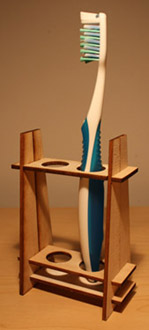
\includegraphics[height=2.2in]{img/flat-a.jpg}
}
\hspace{1cm} \subfloat[] {
    \label{fig:flat-b}
    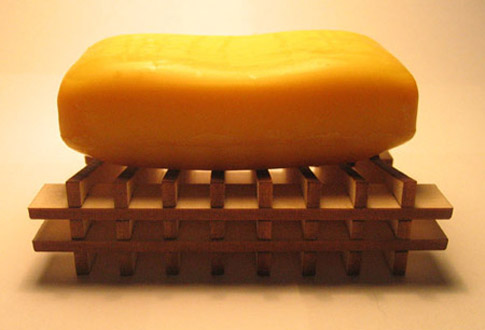
\includegraphics[height=2.2in]{img/flat-b.jpg}
}
\caption{Household objects made with a laser cutter.}
\label{fig:flat}
\end{figure}

\subsection{Conversational Sketch-based Interaction}

The premise of interactive systems is that there is an ongoing
``conversation'' between the user and computer. In sketch-based
systems, users ``speak'' with a stylus; computers ``talk back'' with
graphics. Just as humans have social norms for engaging in
conversation that allow us to talk to people we have not met before,
there should be norms for human-computer interaction in calligraphic
systems so our experience from one application can be used in the
next.

Olsen~\cite{olsen-ui-research} argues the dominant paradigm of ``one
display, one keyboard, one mouse'' hinders progress in interactive
systems that use alternate hardware configurations. There is no
standard for set of interaction techniques and idioms for sketch-based
systems, where hardware is a pen-sensitive display and stylus. In
recent years, researchers have begun to give more attention to
interaction aspects of sketch recognition-based user interfaces, but
the extent of this work remains limited.

For each of the several technical challenges in sketch-based systems
research there is a human component. Segmentation and recognition are
concerned with perceptual and semantic interpretation, which is
inevitably wrong on occasion. When does the system attempt to
recognize input? How detailed must the recognition be in order to
match the user's intentions? What salient aspects are to be
recognized? How does the system tell the user what has been
recognized? When should this occur? How can the user work with the
system to recover from mistakes?

The answer to these questions begins with ``it depends on what the
user is trying to achieve.'' In the proposed system, ideas are
gradually refined from sketches into manufacturable models. The user's
goals are different early in this process compared with latter
stages. Early in this process the user's goal is to simply record
ideas, possibly to share with other people. The early phase is usually
about \textit{big ideas}. Later, the user's goals might be to add
specific details such as lengths, angles, and how different parts
interact---this phase is about \textit{details}.

\subsection{Proposal Organization}

The remainder of the proposal is organized as follows. First I give a
brief overview of the thesis goals, scope, and methods. Next I give
details on the design domain my system will support. To give a better
sense of the system I intend to build, I then present a motivating
scenario of how the system might be used, and relates many of the
sketch-based interaction techniques. Previous related work on sketch
recognition, sketch interaction, and rapid fabrication is then
discussed. Next I detail my own efforts in sketching and design tools
for fast fabrication. The proposal ends with the thesis contributions,
a discussion of how the system will be evaluated, and a time line for
project completion.

\section{Thesis Summary}

This section summarizes the purpose, scope, and methods of my
dissertation.

\subsection{Thesis Statement}

This thesis will present a coherent set of calligraphic interaction
techniques for iteratively making structured drawings that have enough
detail that objects can be fabricated on a laser cutter. Current
computer design tools impose needless, unnatural complexity on
designers. Sketch-based interaction is chosen because of its
widespread use in thinking about and representing design ideas
quickly. If successful, the sketching techniques will enable
relatively inexperienced designers to design and fabricate meaningful
artifacts.

\subsection{Research Scope}

The tool under consideration here supports novice designers in the
fairly narrow domain of design for 2D laser-cutter fabrication. This
domain is chosen because laser-cut parts typically have some aspects
that require precise measurements. 

The research scope of this project is to develop calligraphic
techniques to facilitate the design of these 2D parts. I will evaluate
these techniques in context of the laser-cutting fabrication design
domain. This domain is chosen because it a 2D environment is easier to
develop than a 3D tool.

\subsection{Methods}

This dissertation will center on iteratively creating a calligraphic
design tool. Development will be based on two sources:

\begin{packed_enum}
\item Prior work: This includes the work of others (largely summarized
  in \cite{johnson-sketch-review}) and my own past work.
\item Iterative evaluation: I will regularly test the system with CMU
  students and other volunteers. 
\end{packed_enum}

\section{New Makers, New Tools}

There is a growing community of self-described \textit{makers} who
design and build many kinds of physical
things~\cite{gershenfeld-fab}. Some are electronic or robotic gizmos,
while others are composed of traditional material but designed or made
with modern technology. The ranks of these ``new
makers''~\cite{gross-new-makers} include mechanical engineers,
industrial designers, artists, computer programmers, architects, and
many others. It is common for these people to be relatively untrained
in aspects of their craft, such as using modeling software, designing
or assembling electronics, or making visually appealing physical
constructions. It is rare to find any individual person that is an
expert in all of these topics, but it is common that a person knows
something about a lot of them.

It is possible that we are beginning to see a shift from an economy
based on mass-production (in factories) to one that includes
mass-customization (in homes and community centers). Rapid fabrication
machines continue to decline in price while improving in quality. It
is conceivable that in the not-so-distant future, small manufacturing
machines will be as common as desktop printers~\cite{economist-fab}. A
new sector of small businesses use rapid fabrication to cater to the
needs of hobbyist designers as well as people that need highly
customized goods (e.g. prosthetic limbs)~\cite{nyt-rapidfab}.

The surge of home manufacturing is made possible by a number of
related factors. First, there is a trend away from a culture of
consumption towards a culture of production. This is most visibly
reflected in the democratization of modern media where the users
become the dominant producers of content (e.g. social networking
systems like Facebook or the game Minecraft). People are once again
beginning to participate in the design of the world around them.

Second, there is a developing support structure for the new makers,
including physical shared space, Internet resources, magazines, and
conferences. \textit{Hacker spaces} are physical locations where
people can meet, share ideas, and work on projects. Hacker spaces
commonly have various tools and supplies available to members. Online
stores such as Sparkfun and model sharing sites like Thingiverse and
3D Warehouse give hackers easy access to supplies. There are several
Internet-based companies (e.g. Pokono) that offer fabrication
services. O'Reilly's \textit{Make Magazine} is a popular periodical
catering to this community. O'Reilly also puts on several
\textit{Maker Faire} gatherings every year where physical hackers can
meet.

Last, physical hacking is made accessible by the increasing
availability and affordability of rapid fabrication machines like 3D
printers, CNC mills, and laser cutters. This work focuses on projects
that use laser cutters. Figure~\ref{fig:prices} shows prices for a
comparable~25-Watt,~16''x12'' laser cutter model from Universal Laser
Systems (these values were found on hobbyist web forums). While these
data may not be exact, they do show the price of desktop laser cutting
machines has been cut by almost half in the past ten years. While
still out of reach for most people to afford, they are becoming
inexpensive enough for schools and hacker spaces to own.

% Price information: 
% 2001: 12,900 (ULS 25 watt)
% 2006: 9,995 (ULS 25 watt)
% 2010: 8,500 (ULS 25 watt)
% 2011: 6,850 (ULS 25 watt)
%
%   http://www.rcgroups.com/forums/showthread.php?t=16912 claims that
%   a 25-watt model from Universal Laser systems cost $12,900. Several
%   comments in that thread are in line with that price estimate for
%   home-garage-lab use.
%   http://www.microgeo-usa.com/ProductDetails.asp?ProductCode=universal-laser-VLS2.30
%   currently prices the ULS 25 watt 16x12 unit as costing $6,850.

% http://55-website.com/xo1/ulsinc/english/PDFs/EJ_VL_Article_Reprint.pdf is a press article from 2006 that prices the 25 watt laser at 10,000
\begin{figure}[h] %  figure placement: here, top, bottom, or page
   \centering
   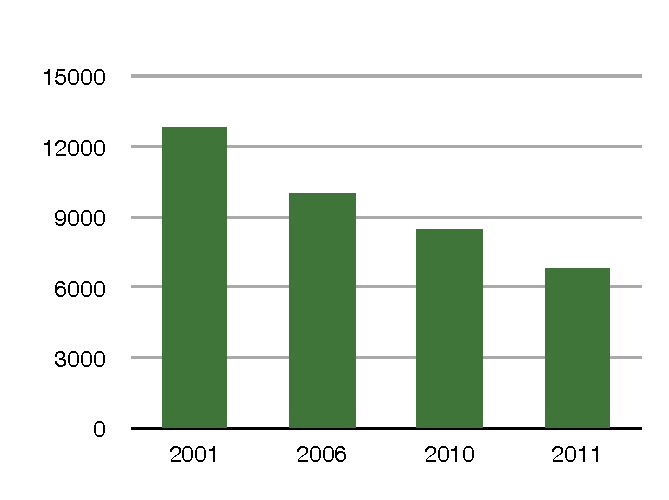
\includegraphics[width=3in]{img/prices.pdf} 
   \caption{Declining prices of Universal Laser Systems 25-Watt 16x12
     inch laser cutter (US Dollars).}
   \label{fig:prices}
\end{figure}

\subsection{Current Design Practices}

\begin{figure}[h] %  figure placement: here, top, bottom, or page
   \centering
   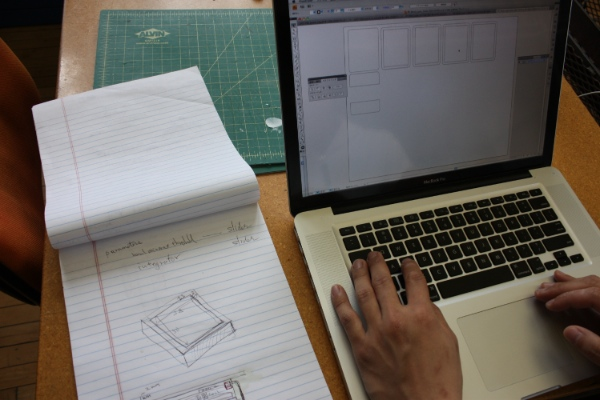
\includegraphics[width=4in]{img/translate-sketch-to-computer.jpg} 
   \caption{A common part of designing for laser cutters: translating
     a hand-made sketch to a computer modeling tool. The sketch
     includes a 3D depiction of the result, with important dimension
     values written down.}
   \label{fig:translating-to-computer}
\end{figure}

Laser cutters (and other rapid fabrication machines) are a relatively
new addition to the design studio. Further, many of the people using
laser cutters are avocational designers that lack formal design
education.

I am currently conducting interviews and observations to better
understand how people think about, model, and make things using laser
cutters. In addition to these interviews I have several years of
exposure and some direct experience on this topic.

\subsection{Laser Cutters and Fabricated Output}

A laser cutter can be thought of as a very fast, strong, and precise
automated razor blade. They cut through flat material (paper, wood,
plastic, metal, etc.) from directly above.

Some items can be made entirely with a laser cutter. These projects do
not involve other machines or material, aside from the occasional
screw or glue. Other projects might be made partly with a laser
cutter, and partly with other machines. Sometimes an artifact is
designed with to allow it to interact with another object that already
exists. This places additional constraints on the design because it
must conform to existing measurements. The car-mounted smart phone
holder in Figure~\ref{fig:phone-holder} is one such example. If we are
given another similar device with slightly different dimensions, we
might simply change some parameters and cut another holder.

\begin{figure}[h] %  figure placement: here, top, bottom, or page
   \centering
   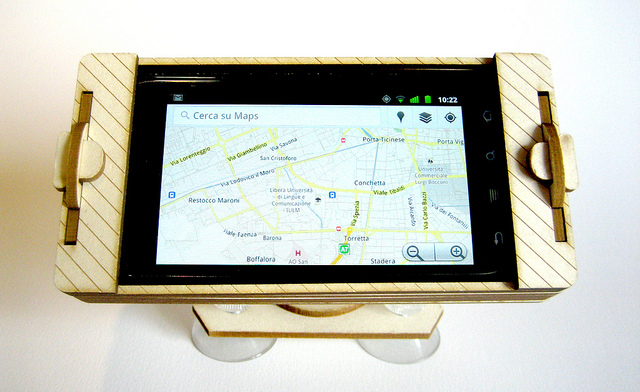
\includegraphics[width=4in]{img/phone-holder.jpg} 
   \caption{A laser-cut smart phone holder designed to fit around a
     particular device and mounted on the dash of a car (by Davide
     Prato).}
   \label{fig:phone-holder}
\end{figure}

\subsection{Current Tools, Current Problems}

Rapid fabrication hardware requires software. Currently, modeling
tools for rapid fabrication are almost exclusively designed for
professional, expert users. The personal computing industry was only
able to take off when intuitive interfaces were developed that allowed
ordinary people to use them. If rapid fabrication is to become common,
software modeling tools must be made accessible by ordinary
users~\cite{lipson-homefactory}.

Today, designers can choose among several modeling tools for laser
cutter projects. As a minimum requirement, the tool must be able to
produce a vector graphics file, where colors indicate which action the
laser takes (e.g. cut through material or etch into it). Adobe
Illustrator is the most commonly used package. Others include Rhino,
InkScape, AutoCAD, and SolidWorks.

Illustrator is a general-purpose vector graphics tool. Specialized
design tools like Rhino or SolidWorks are perhaps more appropriate for
this kind of modeling, but many people are already familiar with
Illustrator from other 2D vector graphics editors. 

I interviewed designers to find out more about their work practices
and better understand how they use their tools. They have
substantially different backgrounds: all have training in some form of
design, ranging from mechanical engineering to graphic design to
architecture. I began by asking each person to describe how they
work. Each designer was able to show me sketches or videos of their
work. While there are subtle (and some substantial) differences in
their processes, each followed the following pattern.

They begin by thinking about a problem and making drawings by
hand. Some sketches are made to think about how to frame the project
(what is it for), while others help reason about how to make it (how
it works, how it fits together). Some designers explicitly noted that
sketching is a necessary part of the process; it would not be possible
to move forward without making freehand drawings. When the idea is
reasonably well-formed they will implement the model with a software
tool. It is common for this to involve translating a hand-made sketch
to a computer model (Figure~\ref{fig:translating-to-computer}). 

Following the interview about their work practices, I gave
participants a sketch (Figure~\ref{fig:interview-sketch}) and asked
them the implement it using their software tool of choice. The purpose
of this task was to learn what problems people met when executing the
common task of translating a sketch to a computer model.

\begin{figure}[h]
\centering 
\subfloat[The part users set out to replicate.] {
  \label{fig:interview-sketch-1} 
  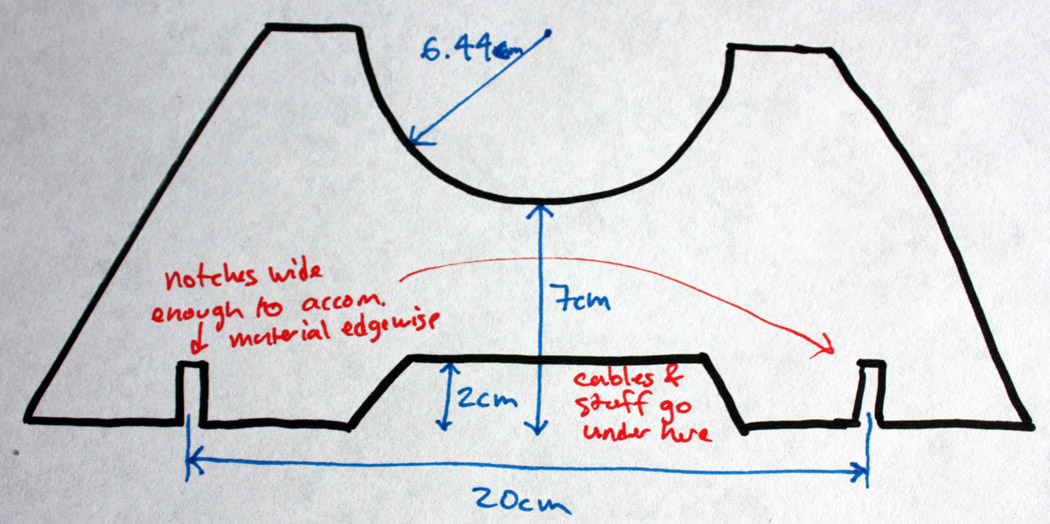
\includegraphics[width=0.5\linewidth]{img/laser-me-1.jpg}
}
\hspace{1cm} \subfloat[Drawing of how the part is used in context.] {
    \label{fig:interview-sketch-2}
    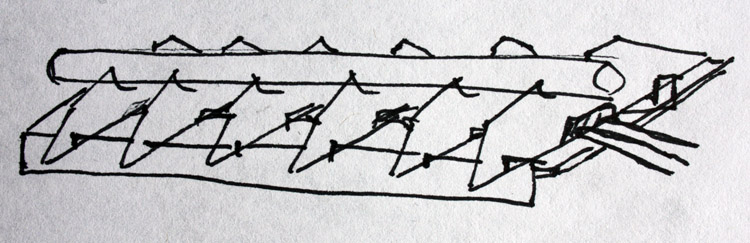
\includegraphics[width=0.5\linewidth]{img/laser-me-2.jpg}
}
\caption{Sketches given to participants to implement in modeling software.}
\label{fig:interview-sketch}
\end{figure}

To design an object suitable for laser cutting, participants used
Illustrator (3 users) or Rhino (1 user). In all cases, a designer's
strategy involved a number of common activities: creating or editing
boundaries, aligning or snapping items, using guide lines or reference
points, measuring distances, specifying or changing lengths and
angles, and creating finished ``cut files'' to send to the laser
cutter. These tasks are in addition to selecting/deselecting, zooming,
panning, and so on.

Participants in this experiment spent a good deal of time on operating
overhead. Overhead includes (1) trying to find the appropriate tool
for the next task, and (2) recovering from errors made when the wrong
tool was selected, or (3) when the tool did not behave consistently
with the user's intention. I have not performed an analysis of the
low-level actions people performed, however I estimate that in my
experiments, more than 50\% of a designers time is spent this way.

For example, one user was aware of Illustrator's ``Path Finder'' tool
and wanted to use it. This user searched the program's menu structure
and hovered over buttons to read tool tips before finding it. Next,
the designer invoked various functions of the Path Finder, using the
keyboard shortcut to undo after each attempt, as he searched for the
correct mode within the Path Finder's subcommand palette. This process
lasted approximately 80 seconds before finally being able to continue.

Participants used the Undo function routinely. The dominant use of
this was to revert after making a single failed attempt to edit some
element. There were a few instances where the designer believed their
current approach was flawed in such a way that it would be better to
back up several dozen operations because a single decision early on
was now observed to be problematic. This is consistent with the study
by Akers \textit{et. al} on the use of undo~\cite{akers-undo}.

One may argue that the problems associated with operating overhead can
be solved by experience or by addressing particular usability
problems. Obviously, masterful Illustrator or Rhino users exist and
would have no problem executing the design task from my
experiment. However, the target audience for this research is
avocational users, not experts. Cooper argues that the set of people
that are truly expert users is not only quite small, it also changes
over time \cite{cooper-inmates}. A person might maintain expert status
for some time, but eventually stops using the program as often, and
eventually becomes an intermediate user, and will generally remain an
intermediate user.

This notion of \textit{perpetual intermediates} is evident in the
designers I interviewed. One participant was a trained graphic
designer and (according to the user's peers) was an Illustrator
expert. However, this designer used some rather strange strategies
during the translation task. In order to remove an unwanted line, this
designer chose to create an opaque white rectangle to obscure it,
rather than erase it. (``Don't tell anyone I did this'', he said at
the time).

Similar episodes are common: a person \textit{should} know the
`correct' action, but takes an alternate approach. The alternate way
may achieve the intended effect, but it might be less efficient (more
operations, longer execution time) or it might introduce unwanted
complexity (e.g. invisible white objects in the model).

\subsection{Implications for Design}

The design observations described above account for a relatively small
slice of hackers designing for laser cutters. It would be unwise to
base an entire research agenda on these few interviews. However, the
current proposal is based on much more than these observations. I have
several years of experience working in an environment where both
undergraduate and graduate students made things with rapid fabrication
machines (including a laser cutter). The recently conducted interviews
validate the observations I have been making for years: current design
tools are hard to learn, provide poor interaction for novice or
occasional users, and do not support idea exploration or informal
representation that is so important during early design.

HCI practitioners often conduct usability studies to uncover
particular problems in applications. The issues uncovered by these
studies are then addressed by changing the software. This iterative
process continues over years, leading to incremental
improvements~\cite{buxton-sketching}.

The interviews and observations from my study confirm that using
current tools involve a great deal of needless overhead for the target
population. However, rather than use this as a basis for incremental
improvement to existing tools, I am interested in developing new tools
the explore an alternate interaction paradigm that is easier and more
effective for typical non-expert designers.

The ultimate goal of any laser cutter project is to make a final
assembly that is made from laser-cut parts. Based on my interviews
with the designers and my own experience, I identify four supporting
goals that serve the larger practical goal of making finished
laser-cut assemblies. These sub-goals include making rough drawings
used to help structure the problem and possible solutions; adding
precise details to drawings; and supporting quick manufacturing and
editing.

\subsubsection{Supporting Goal 1: Make Rough Representation} 

Designers need strategies to help think about (1) what the whole
assembly should work and look like, (2) what individual pieces should
be made, and (3) how those individual pieces fit together. This is
most commonly done via sketching on paper. Some designers make
rough physical models as well.

Current tools do not make any significant allowance for this goal. The
system proposed here is based on sketching as the primary input
method. This will let users be as rough, abstract, and imprecise as
they like.

\subsubsection{Supporting Goal 2: Make Precise Specification}

Users would like to be able to easily specify some (but not
necessarily all) dimensions. This is the main purpose of most current
modeling tools, though it is often difficult for people to do it
effectively. For example, in the translate task, there are two notches
that are specified to be 20cm apart (refer to
Figure~\ref{fig:interview-sketch-1}). Several participants created
temporary geometry (rectangles and lines) that were set to 20cm long
and placed onscreen. This served as a ruler that the designer could
then use to position the notches. The ruler was then erased.

The proposed tool is somewhat unique in the area of sketch-based
design tools in that it will give users the ability to be quite
precise in identifying dimensions and constraints. It is hoped that
using sketch recognition can allow people to state their intentions
substantially faster than using difficult-to-use structured tools.

\subsubsection{Supporting Goal 3: Rapid Editing and Manufacture}

Participants reported they use a rapid \textit{model-make-evaluate}
loop. They make several versions of objects with the laser cutter
before it becomes final, because it is important to be able hold it in
their hands. This is sometimes to determine if they made an execution
error. Equally as as often, the physical ``rough draft'' is necessary
to evaluate their idea. Laser cutter projects tend to be fairly quick
and inexpensive in comparison to some other fabrication machinery like
3D printing.

Current tools impose clumsy requirements on designers to prepare
models for laser cutting. For example, the cut line color need to have
the RGB tuple $(0,0,255)$, and line thickness has to be ``hair line''
at 0.01mm. Managing this overhead is time-consuming. The proposed tool
will handle this overhead on the user's behalf.

A common problem exposed by making a physical draft is the discovery
that pieces do not fit together properly. Some dimensions (such as
notch widths) must then change. However, changing one dimension might
have unwanted side-effects, causing a cascade of issues the designer
must identify and fix, while trying to avoid introducing new problems.

The proposed modeling tool assumes that the user might change the
shape or parameterization of models later on, and facilitate these
changes without creating more problems along the way. 

\section{Motivating Scenario}

\begin{figure}[] 
\centering
\subfloat[Initial sketches of possible designs (preferred idea is circled).] { 
   \label{fig:initial-sketches}
   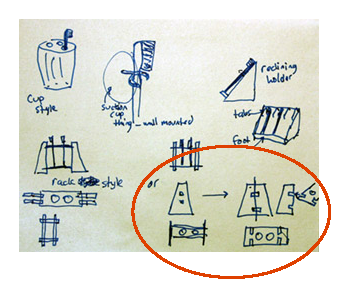
\includegraphics[width=1.8in]{img/physical-sketches-circled-part.pdf} 
}
\hspace{5mm} \subfloat[Sketch of the user's preferred design in
  greater detail.] {
   \label{fig:final-sketch}
   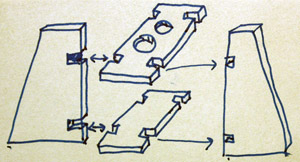
\includegraphics[width=1.8in]{img/final-sketch.jpg} 
}
\hspace{5mm} \subfloat[Final physical output made with a laser
  cutter.] {
   \label{fig:final-physical-output}
   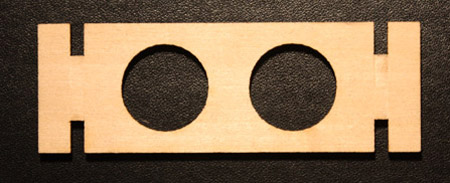
\includegraphics[width=3.2in]{img/final-physical-output.jpg} 
}
\caption{Initial sketches and photograph of one part of the physical
  output.}
\label{fig:physical-sketches}
\end{figure}

This section illustrates how a user might design the toothbrush holder
shown in Figure~\ref{fig:flat-a} using the proposed system. There is
also a video of this process at the URL
\href{http://vimeo.com/17997357}{http://vimeo.com/17997357}.

This narrative is admittedly contrived, because the user is
`designing' a part that has already been completed. It is included in
order to present several proposed interaction techniques as they might
be used together. The scenario in this section does not address the
important interaction techniques that might lead a user to create
several quick drawings used to think about the range of possibilities
(as shown in Figure~\ref{fig:physical-sketches}).

Some toothbrush holders rest on the sink while others are attached to
the wall in some way; some hold a single toothbrush while others
support up to four; some are similar to cups while others resemble
racks. The user makes a variety of drawings (see
Figure~\ref{fig:initial-sketches}) to help think about particular
needs and preferences, and decides to focus on a rack-style holder,
shown in the lower right corner of the initial sketch. This design
features two slats supported at each end by side pieces. Toothbrushes
fit through holes in the top slat and rest on the solid bottom slat.

So far the user had simply been sketching without the benefit of
computation. But now the user is ready to begin thinking about details
of how the object will be made, and the system can let the user supply
information about dimensions.

There are three unique parts used in this design, shown in
Figure~\ref{fig:final-sketch}. To illustrate the interaction
techniques featured in this system, the remainder of this section
focuses on the design of the part with circular holes in it (shown in
Figure~\ref{fig:final-physical-output}). Figures
\ref{fig:ix-draw-bounds}--\ref{fig:ix-draw-guides} depict the design
process.

The user realizes that toothbrush holders come in many sizes, and it
is not completely apparent what the ``right'' dimensions are. Some
properties like width and depth should be parametric, which allow the
model to produce objects in a variety of sizes. Much of the following
activity is guided by the desire to retain flexibility in the model.

The user begins drawing the part as a rectangle. Even though the user
knows the finished slat will have notches cut from several locations,
it is easy to begin by drawing it as a rectangle and removing the
material for the notches later. The user asks the system to interpret
the drawing, and the system replaces the input with a beautified
rectangle~\cite{pavlidis-beautifier}.

The slat features four notches, each of the same size. To make these
the user begins by drawing just one. A pen stroke that begins and ends
outside a part, but traverses a part boundary will remove material
(see Figure~\ref{fig:ix-remove-from-edge}). This cutting gesture has
been used in earlier systems like Teddy~\cite{igarashi-teddy}.

Next the user would like to add dimension details to the
notch. Because the notch is relatively small on the screen, it is
helpful to zoom in (Figure~\ref{fig:ix-zoom-pan}). Zooming is
performed by a double-circle gesture, borrowing the zooming
technique from Lineogrammer~\cite{zeleznik-lineogrammer}. Clockwise
and counter-clockwise gestures zoom in and out respectively. For a few
moments after zooming, a widget appears that lets the user pan to the
desired location.

The user would like to parameterize the notch dimensions so they may be
changed later by name. To parameterize a length, the user draws a line
with arrows on both ends near the desired line segment, and labels it
with writing (Figure~\ref{fig:ix-notch-param}).

The first notch's geometry should be replicated for the next
three. The user can give the system a
\textit{hint}~\cite{mcdaniel-gamut} by selecting existing
elements. The selection is used as a recognition candidate for the
next editing operations---if the user sketches something that
resembles a recently formed selection, the likelihood the user is
replicating the selection is boosted. The user selects the notch by
tracing over it. The selection is graphically acknowledged. Next the
three more notches are drawn at the appropriate places. The
\textit{nd} and \textit{nw} parameters are implicitly copied from the
original to the other notches because they were part of the hint (see
Figure~\ref{fig:ix-hints}).

The user proceeds to give names to the height and width lengths. In
addition the width is given a value, expressed in terms of height (see
Figure~\ref{fig:ix-set-params}). This updates the drawing to reflect
the new width as a function of current height.

Designers often use external tools such as straight edges, French
curves, or stencils when precision is desired. Alternately, people
might lightly draw \textit{construction lines} that guide subsequent
drawing activity~\cite{company-sketching-in-engineering}. The user
would like to draw two circles equidistant from the center of the
slat. To precisely indicate the center of the part, the user draws two
construction lines through the midpoints of two sides
(Figure~\ref{fig:ix-guide-lines}). The designer uses these guides
to place ``fat dots'' in several locations.

The user now wonders if three holes might fit, so two additional
circles are made without using guides. The user decides to stick with
the two-hole design, so the two new holes are erased using a
scribble-out gesture (Figure~\ref{fig:ix-erase}). It is inevitable
that the system's interpretations will occasionally conflict with the
user's intentions. Rather than aiming for perfect recognition (which
is impossible due to ambiguity) this system aims to enable users to
easily recover from such recognition conflicts by providing
appropriate interaction techniques.

The user continues to work, using interaction techniques already
described to parameterize the distance between the center of the part,
and the center of the holes. The user also draws one point where one
of the hole boundaries will be (Figure~\ref{fig:ix-combined}).

The user can hide non-boundary elements like parameters and
construction lines and view the drawing (Figure~\ref{fig:ix-final})
before making the part on a laser cutter. Compare this with the final
output shown earlier in Figure~\ref{fig:final-physical-output}.

\newpage
\newgeometry{left=0.75in,right=0.75in,top=1in,bottom=1in}
\twocolumn

\begin{figure}[] 
\centering
\subfloat[] { 
   \label{fig:ix-draw-bounds-1}
   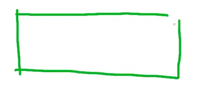
\includegraphics[width=1.35in]{img/ix-draw-bounds-1.png} 
} \subfloat[] {
   \label{fig:ix-draw-bounds-2}
   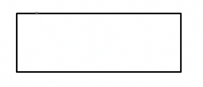
\includegraphics[width=1.35in]{img/ix-draw-bounds-2.png} 
}
\caption{System identifies and rectifies closed shapes.}
\label{fig:ix-draw-bounds}
\end{figure}

\begin{figure}[] 
\centering
\subfloat[] { 
   \label{fig:ix-remove-from-edge-1}
   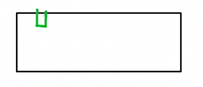
\includegraphics[width=1.35in]{img/ix-remove-from-edge-1.png}
} \subfloat[] {
   \label{fig:ix-remove-from-edge-2}
   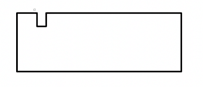
\includegraphics[width=1.35in]{img/ix-remove-from-edge-2.png} 
}
\caption{Remove (or add) material with gestures that cross the part
  boundary.}
\label{fig:ix-remove-from-edge}
\end{figure}

\begin{figure}[] 
\centering
\subfloat[] { 
   \label{fig:ix-zoom-pan-1}
   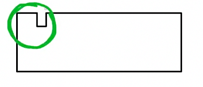
\includegraphics[width=1.35in]{img/ix-zoom-pan-1.png} 
} \subfloat[] {
   \label{fig:ix-zoom-pan-2}
   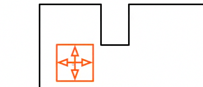
\includegraphics[width=1.35in]{img/ix-zoom-pan-2.png} 
}\\
 \subfloat[] {
   \label{fig:ix-zoom-pan-3}
   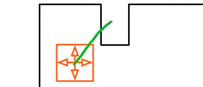
\includegraphics[width=1.35in]{img/ix-zoom-pan-3.png} 
} \subfloat[] {
   \label{fig:ix-zoom-pan-4}
   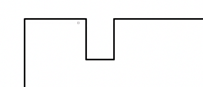
\includegraphics[width=1.35in]{img/ix-zoom-pan-4.png} 
}
\caption{Double-spiral gesture zooms in (clockwise) or out
  (counter-clockwise)~\cite{zeleznik-lineogrammer}. Pan widget appears
  after zoom gesture.}
\label{fig:ix-zoom-pan}
\end{figure}

\begin{figure}[] 
\centering
\subfloat[] { 
   \label{fig:ix-notch-param-1}
   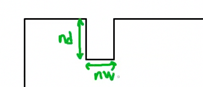
\includegraphics[width=1.35in]{img/ix-notch-param-1.png} 
} \subfloat[] {
   \label{fig:ix-notch-param-2}
   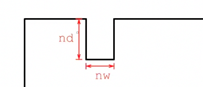
\includegraphics[width=1.35in]{img/ix-notch-param-2.png} 
}
\caption{Make length parameters with double-headed arrows and text.}
\label{fig:ix-notch-param}
\end{figure}

\begin{figure}[] 
\centering
\subfloat[] { 
   \label{fig:ix-hints-1}
   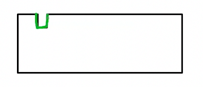
\includegraphics[width=1.35in]{img/ix-hints-1.png} 
} \subfloat[] {
   \label{fig:ix-hints-2}
   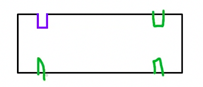
\includegraphics[width=1.35in]{img/ix-hints-2.png} 
}
\caption{Make hints by selecting elements. The hint guides
  interpretation.}
\label{fig:ix-hints}
\end{figure}

\begin{figure}[] 
\centering
\subfloat[] { 
   \label{fig:ix-set-params-1}
   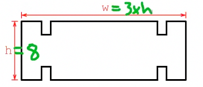
\includegraphics[width=1.35in]{img/ix-set-params-1.png} 
} \subfloat[] {
   \label{fig:ix-set-params-2}
   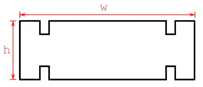
\includegraphics[width=1.35in]{img/ix-set-params-2.png} 
}
\caption{Set parameter values. Model updates to reflect new
  constraints.}
\label{fig:ix-set-params}
\end{figure}

\begin{figure}[] 
\centering
\subfloat[] { 
   \label{fig:ix-guide-lines}
   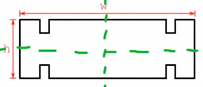
\includegraphics[width=1.35in]{img/ix-guide-lines.png} 
} \subfloat[] {
   \label{fig:ix-guide-dots}
   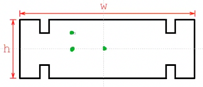
\includegraphics[width=1.35in]{img/ix-guide-dots.png} 
}\\
 \subfloat[] {
   \label{fig:ix-guide-circles}
   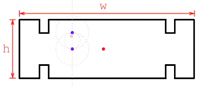
\includegraphics[width=1.35in]{img/ix-guide-circles.png} 
}
\caption{Guides facilitate accurate
  drawing. Guidelines~\subref{fig:ix-guide-lines} and reference
  points~\subref{fig:ix-guide-dots} drawn as indicated; circular
  guides~\subref{fig:ix-guide-circles} made by selecting reference
  points.}
\label{fig:ix-draw-guides}
\end{figure}

\begin{figure}[] 
\centering
\subfloat[] { 
   \label{fig:ix-erase-1}
   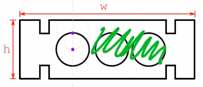
\includegraphics[width=1.35in]{img/ix-erase-1} 
} \subfloat[] {
   \label{fig:ix-erase-2}
   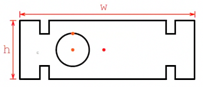
\includegraphics[width=1.35in]{img/ix-erase-2} 
}
\caption{The user draws two holes but changes their mind and erases
  them with a scribble gesture.}
\label{fig:ix-erase}
\end{figure}

\begin{figure}[] 
\centering
\subfloat[] { 
   \label{fig:ix-combined}
   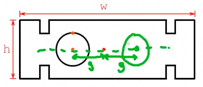
\includegraphics[width=1.35in]{img/ix-combined.png} 
} \subfloat[] {
   \label{fig:ix-final}
   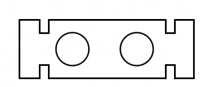
\includegraphics[width=1.35in]{img/ix-final.png} 
}
\caption{Combine techniques to finish part.}
\label{fig:ix-final-steps}
\end{figure}
\restoregeometry
\newpage
\onecolumn
\doublespacing
\section{Related Work}

While ``the design process'' has important differences from domain to
domain, nearly all designers sketch. The ease of freehand drawing
allows people to quickly externalize ideas to analyze their
consequences, as well as to help see new
solutions~\cite{lawson-designers-think,goldschmidt-dialectics}. Many
design professions formalize the importance of sketching by making it
central to the schooling: architects, industrial and interaction
designers, and mechanical engineers are all explicitly taught to
sketch. And even though sketching is not taught in other design
domains (like software engineering), freehand drawing is still
commonly done. Even people who consider themselves non-designers make
quick drawings to help think through everyday problems like how the
furniture in their house might be arranged. Freehand drawing is done
by people of all ages~\cite{goldschmidt-backtalk} and experience
levels~\cite{suwa-analysis-students}.

The prior literature on technical aspects related to this project can
be described in three categories: sketch recognition, calligraphic
interaction, and rapid fabrication.

\subsection{Sketch Recognition}

Ideally, computers would understand sketches as readily as
people. This is of course a very difficult problem of artificial
intelligence. Therefore, researchers often restrict the problem by
obliging users to draw shapes in prescribed
ways~\cite{rubine-recognizer,wobbrock-dollar}, or by limiting the user
to work in specific domains with fairly small visual vocabularies (on
the order of tens of meaningful primitives). Further improvements are
made if the system can correctly identify contextual clues (often
driven by domain semantics) to prune unlikely
interpretations~\cite{gross-ecn-uist,do-phd-thesis}.

Many sketch recognition approaches include at least two distinct
tasks. The first is primitive ink parsing (also known as
segmentation). This process interprets raw user input (time-ordered
point sequences) into atoms such as straight lines, curves,
intersections, and corners \cite{paulson-paleosketch}. In systems that
recognize multi-stroke elements, this step is also usually responsible
for determining which atoms should be considered together. Segmenters
often leverage temporal
data~\cite{sezgin-masters-early-ink,wolin-smr}, spatial
data~\cite{kara-recognizer-cg}, or both~\cite{cates-phd-thesis}.

The second task is to analyze these atoms to perform
recognition. Recognition accuracy is dependent on the quality of the
primitive ink parsing. To increase robustness and accuracy, some
techniques supply multiple possible segmentations to the
recognizer~\cite{alvarado-dynamic-bayes}.

Design sketches from most domains combine diagrammatic ink and written
language. It is helpful for the system to identify what is writing and
what is not~\cite{shilman-discerning-structure}. If done correctly,
such meta-recognition can ease the recognition task by reducing the
amount of input to interpret.

\subsection{Calligraphic Interaction}

Applications often interpret user input differently depending on which
\textit{mode} the program is in (e.g. line mode, circle mode, text
mode, and so forth). This simplifies the computer's task because it is
unambiguous how to interpret user input. But this complicates the
user's task because they must manage modes while designing. 

One way to make mode changing transparent is to infer the user's
intention. The inferred mode protocol~\cite{saund-inferred-mode}
analyzes user input to determine if user input is unambiguous enough
for action to be taken. When ambiguity exists, the system might
mediate by asking what was intended, or take no action and wait for
additional input~\cite{mankoff-burlap}.

Another way of easing the problem of mode is to make it easier for
users to change between them. This might involve buttons pressed with
the non-dominant hand, or with pen gestures such as dwell or pigtail,
or by using pressure\cite{li-mode-switching}.

Drawn gestures can be powerful, but users must first know of their
existence. Some gestures seem easy enough that people do not
necessarily need to ``learn'' them (e.g. scribble over something to
erase it), but many gestures are hard to remember and might be nearly
impossible to discover without assistance. GestureBar is a novel
approach to let users discover and practice
gestures~\cite{bragdon-gesturebar}.

Last, mode can be managed as it is in traditional applications, where
people use on-screen widgets. These widgets may be present at all
times~\cite{forbus-nusketch-battlespace}, invoked via
gesture~\cite{grossman-hover-widgets,kurtenbach-marking-menus} or by
placing the pen near onscreen
ink~\cite{marinkas-shadowbutton,grossman-handle-flag}.

Design sketches often involve a combination of text and pictures. In
situations where the computer should recognize text (or at least
recognize which ink specifies writing) it is necessary to distinguish
between what is text and what is not. One approach is to automatically
classify input as text or non-text based on a statistical analysis of
its visual properties \cite{patel-detect-text}. Another approach is to
ask the user to specify what is text by performing a gesture. This was
the approach taken by the developers of
Lineogrammer~\cite{zeleznik-lineogrammer}.

The proposed work is similar to Lineogrammer and the ParSketch
system~\cite{company-sketching-in-engineering,naya-parsketch} in
several key respects: they both offer the ability to create precise
drawings by using sketch and gesture recognition, and they both eschew
modal input when possible. The proposed work integrates many more
sketch- and pen-based interaction techniques. Also, because it is in
support of machined output, it is necessary that the drawing give
enough detail that objects can be manufactured.

\subsection{Sketching for Rapid Fabrication}

Sketching has long been a subject of study by makers of physical
things. Leonardo da Vinci's legendary sketchbooks are an early example
of the utility of sketching for both thinking and for
specifying. Demonstrations of the earliest computer-based sketching
system, Sketchpad~\cite{sutherland-sketchpad}, mostly focused on
drawing machinable parts.

Until fairly recently, many systems for 3D modeling or fabrication
have used the term ``sketching'' as shorthand for ``quick'' in
comparison to traditional CAD modeling
interfaces~\cite{bloomenthal-sketch-n-make,pugh-thesis-viking,zeleznik-sketch}. Google
SketchUp is a commercial example of this.

Many researchers interested in sketch input for designing physical
objects have been concerned with recognizing 3D drawings,
e.g.~\cite{lipson-correlation,masry-3d-sketch}. Such work focuses on
interpreting the 3D geometric meaning of a finished 2D sketch. In a
sense, that approach assumes that the designer's creative work has
concluded and the job of the computer is to translate the drawing into
a 3D model. This contrasts with interactive approaches that aim to
support an ongoing conversation between the human and computer. A
conversational system tacitly acknowledges that the user's ideas are
not fully formed from the onset, but become progressively clearer and
more defined as they work.

With the availability of prototyping machines, sketch-based systems
for fabrication are beginning to receive attention. The Furniture
Factory accepts 2D sketch input that is recognized as a 3D
configuration of planes~\cite{oh-fab}. The user adds pieces
incrementally, so there is no need to make a complete sketch all at
once. The system automatically computes how these planes can be joined
together and generates a series of 2D pieces that to be produced with
a laser cutter.

Saul's Sketch Chair \cite{saul-sketch-chair} is another sketch-based
system for generating furniture. It lets users sketch the contours of
a chair's seat and back rest, and using a different drawing mode, add
legs. The system includes a sophisticated physical simulator to let
the designer explore its physicality (for example to determine if it
will remain upright), and if it will be comfortable. It also allows
designers to change subtle properties of curves using onscreen control
handles. My proposed system differs from Sketch Chair in two important
respects. First, Saul's system presumes the user is making a chair or
chair-like object, and provides highly specialized software analysis
tools. To borrow from Henry Ford, you can make anything you want, as
long as it is a chair. My system is more general, so the range of
possibilities with my tool is wider. Second, Sketch Chair (and many
systems like it) constrain designers to using a small set of part
junction types. My system does not propose to include pre-specified
junction types. This is both liberating (because designers are free to
chose whichever type they want) but also encumbering (because they
must design the junctions themselves).

Plushie lets people make bulbous textile objects such as plush toys or
balloons~\cite{mori-plushie}. Users iteratively design objects by
drawing object boundaries or giving editing commands by sketched
gesture. The interaction is based on prior systems in the Teddy family
tree~\cite{igarashi-teddy}.

\section{My Prior Work}

The Designosaur~\cite{oh-fab} is a prototype system for kids to design
their own wooden dinosaur ``skeletons''. Users begin by drawing
individual bone outlines and specify notch locations where the bone
joins another. To support this, the user can name bones and apply
those names to indicate how bones fit together.

We noticed that editing bone boundaries presented some challenges.
First, dinosaur model bones are frequently symmetric (e.g. ribs or
vertebrae). The system featured a simple ``mirror mode'' that helped
users make the parts symmetric about the horizontal or vertical axes.
Second, it is useful to be able to change the shape of bones
easily. To tweak the bone curvature without redrawing, we invented a
local editing technique called Flow selection.

Flow selection~\cite{johnson-flow-selection} is a modeless, time-based
selection and editing technique for picking a region of a 2D boundary
and changing its shape. It is especially useful in cases such as the
Designosaur when organic curves are desired. The user sets their
stylus down near a boundary and holds it still as a selection begins
to form. An apt metaphor is that the pen is ``heating'' the region,
which is strongly selected near the pen, and progressively less
selected as distance increases along the boundary path. Then the user
moves the pen to begin reshaping the selected region---the more
strongly selected the ink, the more it moves. The user may lift their
pen up to end the operation, or hold it still once again to smooth the
region. This is helpful in cases where the user input includes
unwanted bumps or jagged lines.

Whereas the Designosaur is based on sketching, the follow-on system is
based on programming. FlatCAD is a system for designing and
manufacturing things on a laser cutter by writing programs in a
language called FlatLang~\cite{johnson-flatcad}.  FlatLang features a
``flying turtle''---a 3D version of the LOGO turtle---which lets the
user compose 3D models of objects built from flat pieces. This helps
users to specify and see how parts will fit together. FlatCAD made it
easy to design everyday items using parameters, so the same model
(FlatLang program) could be used to generate a variety of physical
objects. The objects shown earlier (Figure~\ref{fig:flat}) were made
using FlatCAD.

My experience with the Designosaur sparked an interest in sketch-based
interaction techniques, while FlatCAD kindled an interest in tools for
making precise, machinable models. The Designosaur lacks the ability
to make precise edits: make a notch \textit{here} facing \textit{this
  direction}; make \textit{this} collinear with \textit{that}; and so
on. FlatCAD addressed this issue but introduced roughly the opposite
problem: it is impossible to be non-specific or tentative when writing
a FlatLang program. The current proposal is an effort to bridge the
gap between the positive aspects of sketching (rough, tentative,
fluid) with the positive aspects of FlatCAD-style modeling (precise,
specific, parametric).

To better understand the space of sketch-based design tools, I
co-authored an extensive survey with my thesis
committee~\cite{johnson-sketch-review}. This survey was motivated by
the question: \textit{After forty years of research on computational
  support for sketching, why there are so few real world applications
  of this technology?} In my personal view, a significant reason is
that we lack appropriate sketch-based interaction techniques. The
proposed work seeks to establish a better understanding of what
constitutes good sketch-based interaction. The proposed system is a
vehicle for this research.

%% TODO: Maybe a screen shot of Designosaur or the output, and for
%% FlatCAD.

%% TODO: Need to add a few paragraphs for (1) Skrui Draw, (2) my Ouyang
%% writing recognizer implementation, (3) what I have of SkruiFab so far.

\section{Evaluation}

Interaction techniques are challenging to evaluate. There is a
tradition in human-computer interaction to evaluate novel interaction
techniques in a laboratory setting. People perform simple tasks
designed to evaluate the technique in isolation. While this evaluation
approach has its benefits, it avoids the reality that people use
interaction techniques \textit{with other techniques} and \textit{in
  service of a larger purpose}. 

Therefore, the proposed system will be evaluated as a whole, rather
than testing isolated pieces. The proposed system offers a set of
techniques that are intended to work harmoniously together to support
users in the realistic goal of designing household objects using flat
material. To test if the system works as intended it will be compared
with existing tools such as Illustrator, SolidWorks, SketchUp, Rhino,
as well as plain pencil and paper.

The evaluation criteria in this ``whole system'' analysis focus on
what users are able to do (or not do) that would be possible with
traditional structured design software. What is possible to create
using this system? What is \textit{not} possible? What are the common
interaction problems or errors? Do users tend to develop particular
usage patterns that might be exploited? Or do usage patterns indicate
underlying flaws with the system?

Iterative evaluation will be used throughout the development
process. Therefore, the exact list of features (and perhaps evaluation
criteria) must be flexible. Test participants will be asked to design
and fabricate a functional object such as the toothbrush holder
in~Figure\ref{fig:flat-a}. Object choice will depend on the system's
capabilities at the time of testing.

This whole-system approach will allow me to gauge several factors that
compare the proposed system with existing WIMP-based tools:

\begin{packed_enum}
\item Time taken for design and fabrication
\item Number of unique design ideas (as measured
  in~\cite{goel-sketches-of-thought})
\item Overall user satisfaction
\item User satisfaction with individual techniques
\item User satisfaction with certain combinations of techniques
\item How ``learnable'' the interaction style is
\item How system supports (or does not support) alternate working
  styles
\item How well tool helps people \textit{think}, \textit{create},
  \textit{explore}, \textit{visualize}, \textit{specify}, and
  \textit{fabricate}
\item User feedback: criticism and suggestions
\end{packed_enum}

This evaluation rubric does not explicitly address technical factors
traditionally found in work done on sketch based systems. These
factors include recognition accuracy or computational complexity of
various algorithms. Measures such as user satisfaction should account
for such aspects: if the system misinterprets input but provides
adequate methods for recovery, recognition accuracy is not a problem.

\section{Contribution}

Currently there are few interaction techniques for sketch-based
interfaces, and even fewer examples of coherent sets of techniques. As
stated earlier, it is desirable to provide a design system in which
the user can do everything without setting down the stylus.

This thesis will explore the space of calligraphic interaction
techniques to support researchers seeking to make sketch-based design
systems in contexts beyond the laser cutter scenario described above.

This thesis will contribute the following:
\begin{packed_enum}
\item A set of calligraphic interaction techniques. Some will be based
  on existing techniques (e.g. Lineogrammer's zoom), others will be
  novel. Here, \textit{technique} is broadly defined to include
  interactive onscreen widgets, gestural phrases, and user interface
  conventions.
\item An analysis of \textit{the contexts and use cases} when each
  technique is appropriate. For example, rectification might be
  appropriate for latter stage design but distracting during early
  exploratory sketching.
\item An analysis of \textit{which techniques} are complementary.
\item Recommendations for developing further techniques.
\item Software engineering implementation details.
\end{packed_enum}

The best interactive systems have discoverable, consistent interaction
techniques working in concert. Companies such as Microsoft and Apple
have user interaction guidelines for various platforms (Windows,
Windows Mobile, OS X, iOS) that give developers standard advice for
developing such systems. Pen- and touch-oriented interaction guides
exist for TabletPCs and (recently) the iPad, but these devices are by
no means sketch-based in that the interaction is still expected to be
largely unambiguous, and requires little interpretation. No guide yet
exists for sketch-based interactive systems. This thesis will provide
a concrete step to providing one.

\section{Time line}

In this section I first describe a short schedule for developing the
sketch-based system, followed by a longer-term schedule for completing
the dissertation. 

\subsection{System Development}
\label{sec:system-development-schedule}

I have already written a good deal of code this project, so it should
not take long to develop a rudimentary prototype. Existing code
includes ink analysis and supported data structures (such as Masry's
Angular Distribution Graph~\cite{masry-3d-sketch} among others) and
Ouyang's PCA-based printed character
recognizer~\cite{ouyang-visual-recog}. External tools will be used
whenever possible.

The following table presents a tentative schedule for system development.

\vspace{12pt}
\begin{tabular}{ | l | c | l | }
  \hline

  \textbf{Milestone} & \textbf{Num. Weeks} & \textbf{Topic} \\

  \hline \hline

  Milestone 1 & 1 week & Primitive stroke analysis to generate constraints \\
  
  Milestone 2 & 1 week & Establish boundary model \\

  Milestone 3 & 1 week & Recognize gestures to add/subtract material \\

  Milestone 4 & 1/2 week & Erase unwanted ink with scribble gesture. \\

  Milestone 5 & 1/2 week & Implement zoom and pan widgets. \\ 

  Milestone 6 & 1 week & Indicate and name linear dimensions. \\

  Milestone 7 & 1/2 week & Indicate and name angular and location dimensions. \\

  Milestone 8 & 1/2 week & Indicate guides (points, lines, circles). \\ 

  Milestone 9 & 1 week & Indicate hints and use them for interpretation. \\ 

  Milestone 10 & 1 week & Indicate parameter values (scalar) \\ 

  Milestone 11 & 1 week & Indicate parameter values (expression) \\

  \hline
  
  & 9 weeks total & \\

  \hline

\end{tabular}
\vspace{12pt}

Throughout this process I will conduct informal user studies to
calibrate my work. Additionally, at each step in the process I will
ensure that the system does what it should by using it to make items
with a laser cutter. 

A common heuristic project managers use to predict completion time is
to multiply the predicted time by three---this brings the expected
duration to 27 weeks, or about six months.

\subsection{Dissertation Schedule}

The schedule for completing and defending the dissertation
follows. Because the completion time for system building has such a
wide spread, best- and worst-case schedules are given.

\vspace{12pt}
\begin{tabular}{ | l | c | p{80mm} | }
  \hline

  \textbf{Component} & \textbf{Num. Weeks} & \textbf{Remark} \\

  \hline \hline

  System Development & 9--27 weeks & Schedule given above in
  section~\ref{sec:system-development-schedule}. \\

  User Interviews & 2--4 weeks & Understand current problems and
  processes. \\

  System Evaluation & 2--4 weeks & Includes modifications based on
  feedback. Concurrent with system development. \\ 

  Dissertation draft & 4--8 weeks & Borrow from literature
  survey~\cite{johnson-sketch-review} and this proposal. \\

  Dissertation revisions & 3--8 weeks & ---\\

  Defense preparation & 2 weeks & ---\\

  \hline

  \multicolumn{3}{|c|}{
    Summary: 9--27 weeks development, 13--26 weeks other = 
    \textit{22--53 weeks total}
  } \\

  \hline

\end{tabular}

\singlespacing\newpage
\bibliographystyle{plain}

\addcontentsline{toc}{section}{References}
\bibliography{sketch-bibliography}

\end{document}

% how do you accellerate the process by which they become good

% where do they spend the most time?

% the multiple undo problem: backing up 3 minutes, fixing for another
% 3 = 6 minute mistake.

% q1: what's the effective role of sketching?

% q2: how to reconcile the rough nature of sketching and the precise
% demands of laser cutters?

% maybe: start with a physical sketch, scanned, as the basis for
% gradually making it structured.

% paul debevec, image use in modeling

% make a taxoomy of the things people make, trying to create on the
% ponoko blog. make a list of 

% Fred Brooks: (no silver bullet)

% accidental: problems that would be fixed over time

% essential: no matter how much better our software gets, we still
% have to deal with them.


